%%%%%%%%%%%%%%%%%%%%%%%%%%%%%%%%%%%%%%%%%
%
% (c) 2020 by Jennifer Laaser
%
% This work is licensed under the Creative Commons Attribution-NonCommercial-ShareAlike 4.0 International License. To view a copy of this license, visit http://creativecommons.org/licenses/by-nc-sa/4.0/ or send a letter to Creative Commons, PO Box 1866, Mountain View, CA 94042, USA.
%
% The current source for these materials is accessible on Github: https://github.com/jlaaser/pogil-polymers
%
%%%%%%%%%%%%%%%%%%%%%%%%%%%%%%%%%%%%%%%%%

\documentclass[instructor,handout]{pogil}

%%%%%%%%%%%%%%%%% DOCUMENT INFORMATION %%%%%%%%%%%%%%%%%%%%%%%%

\copyrightshort{
\includegraphics[width=0.1\textwidth]{by-nc-sa} J. Laaser 2020}

%%%%%%%%%%%%%%%%%%%%%%%%%%%%%%%%%%%%%%%%%%%%%%%%%%%%%%%%%%%%%%%%%
%%%%%%%%%%%%%%%%%%%%%%%%%%%%%%%%%%%%%%%%%%%%%%%%%%%%%%%%%%%%%%%%%

\begin{document}
	
% to change the activity output in the pdf, change this to the file path for the activity you want to include:
%%%%%%%%%%%%%%%%%%%%%%%%%%%%%%%%%%%%%%%%%%
%
% (c) 2018 by Jennifer Laaser
%
% This work is licensed under the Creative Commons Attribution-NonCommercial-ShareAlike 4.0 International License. To view a copy of this license, visit http://creativecommons.org/licenses/by-nc-sa/4.0/ or send a letter to Creative Commons, PO Box 1866, Mountain View, CA 94042, USA.
%
% The current source for these materials is accessible on Github: https://github.com/jlaaser/pogil-polymers
%
%%%%%%%%%%%%%%%%%%%%%%%%%%%%%%%%%%%%%%%%%

\section{Activity Template}
\renewcommand{\figpath}{content/figs}

\textbf{Focus question:} Put a central question for the students to consider through this exercise here.

\subsection{Model 1:  ABC}

Here is the first model for students to consider

% to include images, put them in the folder specified by figpath and then use:
%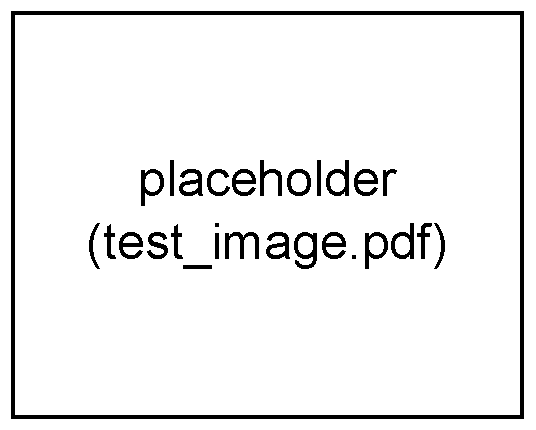
\includegraphics[width=0.8\textwidth]{\figpath/test_image.pdf}

\subsection{Critical Thinking Questions}

	\begin{enumerate}
		\item First question?
		\item Second question?
	\end{enumerate}

\subsection{Model 2: DEF}

\subsection{Critical Thinking Questions}

	\begin{enumerate}
		\item First question?
		\item Second question?
	\end{enumerate}

\subsection{Exercises}

	After class, \textbf{read} the following sections of your textbook:
	
	\begin{enumerate}
		\item First section
		\item Second section
	\end{enumerate}
	
	Then, do the following exercises:
	
	\begin{enumerate}
		\item First exercise
		\item Second exercise
	\end{enumerate}
%%%%%%%%%%%%%%%%%%%%%%%%%%%%%%%%%%%%%%%%%
%
% (c) 2019 by Jennifer Laaser
%
% This work is licensed under the Creative Commons Attribution-NonCommercial-ShareAlike 4.0 International License. To view a copy of this license, visit http://creativecommons.org/licenses/by-nc-sa/4.0/ or send a letter to Creative Commons, PO Box 1866, Mountain View, CA 94042, USA.
%
% The current source for these materials is accessible on Github: https://github.com/jlaaser/pogil-polymers
%
%%%%%%%%%%%%%%%%%%%%%%%%%%%%%%%%%%%%%%%%%

\renewcommand{\figpath}{content/polymchem/freeradical/FRPchemistry/figs}
\renewcommand{\labelbase}{FRPchemistry}

\begin{activity}{Chemistry of Free-Radical Polymerization}

\begin{instructornotes}
	This activity introduces students to concepts related to the chemistry of free-radical polymerization.
	
	After completing this activity, students will be able to:
	\begin{enumerate}
		\item Draw appropriate mechanisms for the initiation, propagation, termination, and chain-transfer steps of a free radical polymerization
		\item Identify common initiators and the fragments that they leave on the ends of polymer chains
		\item Explain why free-radical polymerization typically results in head-to-tail addition of monomers
		\item Explain how different termination modes affect the end-group functionality and chain length of polymers produced by free radical polymerization
	\end{enumerate}
	
	\subsection*{Activity summary:}
	\begin{itemize}
		\item \textbf{Activity type:} Learning Cycle
		\item \textbf{Content goals:} Chemistry of free-radical polymerization
		\item \textbf{Process goals:} %https://pogil.org/uploads/attachments/cj54b5yts006cklx4hh758htf-process-skills-official-pogil-list-2015-original.pdf
			written communication, critical thinking, information processing
		\item \textbf{Duration:} 60 min, including time for discussion
		\item \textbf{Instructor preparation required:} none beyond knowledge of relevant content
		\item \textbf{Related textbook chapters:}
			\begin{itemize}
				\item \emph{Polymer Chemistry} (Hiemenz \& Lodge): sections 3.3.1, 3.3.2, 3.4.1, 3.5.0, 3.8.0
			\end{itemize}
		%\item \textbf{Facilitation notes:}
		%	\begin{itemize}
		%		\item \dots
		%	\end{itemize}
	\end{itemize}
	
\end{instructornotes}


\begin{model}[Initiation]
	\label{\labelbase:mdl:FRPinitchem}

	In a free-radical polymerization, the reactive species is a radical at the ``active'' end of each polymer chain.  Thus, the first step in a free radical polymerization is to generate an active radical species.  We refer to this step as \emph{initiation}.
	
	Shown below are two common chemistries used to generate initiator radicals in free-radical polymerizations:
	
	\begin{enumerate}
		\item Thermal decomposition of azobisisobutyronitrile (AIBN):
	
			\centerline{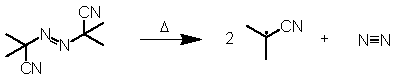
\includegraphics[scale=1.25]{\figpath/Model1-AIBN.pdf}}
			
		\item Thermal decomposition of benzoyl peroxide:
	
			\centerline{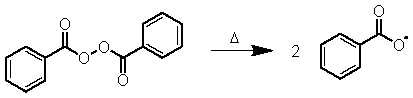
\includegraphics[scale=1.25]{\figpath/Model1-BPO.pdf}}
			
	\end{enumerate}
	
	%Note: this paper addresses the issue of benzoyl peroxide's further decomposition to phenyl radicals: 10.1021/ma00231a042 - it looks like it really is mostly the ester radical that adds about 95% of the time.
	
\end{model}


\begin{ctqs}

	\question On the left-hand side of each reaction, how many molecules are present?  Are any of them radicals?
	
		\begin{solution}[0.5in]
		
			1 molecule; no radicals
			
		\end{solution}
	
	\question On the right-hand side of each reaction, how many molecules are present? Are any of them radicals?
	
		\begin{solution}[0.5in]
		
			2 or 3 molecules; 2 radicals
			
		\end{solution}
	
	\question Briefly describe, in 1-2 complete sentences, what you would need to do to the reaction to generate initiator radicals in a polymerization using AIBN or benzoyl peroxide.
	
		\begin{solution}[1.5in]
			Since these are both thermal decomposition reactions (and show heat, $\Delta$, above the reaction arrow), you would generate initiator radicals by heating the reaction up.
		\end{solution}
		
	\question Ideally, the radical, which we often abbreviate \ce{I^.}, will go on to attack a monomer and start a polymer chain, as shown schematically below:
	
			\centerline{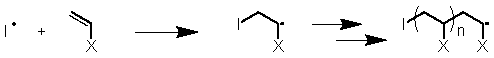
\includegraphics[scale=1.25]{\figpath/Model1-prop.pdf}}
	
		\begin{enumerate}
			\item Does the initiator radical become a permanent part of the polymer chain?  If so, where is it located?
	
				\begin{solution}[1in]
					Yes - it is located at the end of the chain opposite the radical site.
				\end{solution}
			
			 \item Shown below is the structure of a polymer produced by free-radical polymerization:
	
			\centerline{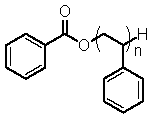
\includegraphics[scale=1.25]{\figpath/Model1-polymstruct.pdf}}
	
			What initiator was used in this polymerization?  In 1-2 complete sentences, briefly explain how you know.
	
				\begin{solution}[1.75in]
					This polymer must have been produced using benzoyl peroxide.  It contains the radical fragment from benzoyl peroxide on the left-hand side.
				\end{solution}
			
			\item If the same polymerization had been carried out using the other initiator shown in Model \ref{\labelbase:mdl:FRPinitchem}, what would the structure of the resulting polymer be?  Make sure to include the relevant end group(s).
	
				\begin{solution}[1.75in]\instructordisplay{
					Replace the benzoyl peroxide fragment with an AIBN fragment:
					
			\centerline{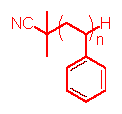
\includegraphics[scale=1.25]{\figpath/Model1-polymstruct-answer.pdf}}
			
				}\end{solution}
				
		\end{enumerate}
		
	\question Some initiator fragments may also undergo side reactions such as the recombination reaction shown below:
	
			\centerline{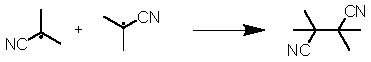
\includegraphics[scale=1.25]{\figpath/Model1-recomb.pdf}}
			
				How do you expect these types of side reactions to affect the overall ``efficiency'' of initiation in a free-radical polymerization? Briefly explain your reasoning in 1-2 complete sentences.
	
				\begin{solution}[1.25in]
					Generally, this should reduce the efficiency of initiation, because it will result in fewer radicals available to initiate new polymer chains.
					
					\emph{Note: generally, only about 30-80\% of generated radicals will actually go on to start polymer chains.}
				\end{solution}

\end{ctqs}



\begin{model}[Propagation]
\label{\labelbase:mdl:FRPpropchem}

	The second important step in a free radical polymerization is \emph{propagation}.  In this step, an active polymer chain radical attacks a monomer and links it to the chain, as shown below:
	
			\centerline{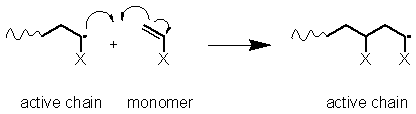
\includegraphics[scale=1.25]{\figpath/Model2-prop1.pdf}}
	
	For convenience, we will often abbreviate the active polymer chain as \ce{P^.}, in which case the propagation step can be depicted as:
	
			\centerline{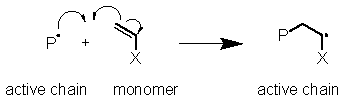
\includegraphics[scale=1.25]{\figpath/Model2-prop2.pdf}}
	

\end{model}

\begin{ctqs}

	\question Briefly describe what happens to the radical in the propagation step shown in Model \ref{\labelbase:mdl:FRPpropchem}.%Does the number of radicals present in the polymerization change during a polymerization step?  If so, how?
	
		\begin{solution}[1.5in]
			The original radical reacts one electron from the double bond on the monomer to form a new single bond.  The remaining electron from the double bond on the monomer forms a new radical site at the end of the elongated chain.
		\end{solution}
	
	\question Does the length of the polymer chain change during a propagation step?  If so, how?
	
		\begin{solution}[1.2in]
			Yes, the length of the polymer chain increases by one monomer.
		\end{solution}
	
	\question In Model \ref{\labelbase:mdl:FRPpropchem}, the radical is shown attacking the less-substituted side of the monomer (often called its ``tail'').  
	
		\begin{enumerate}
			\item This process is shown explicitly for polystyrene, below:
	
			\begin{solution}[1.2in]\studentdisplay{
				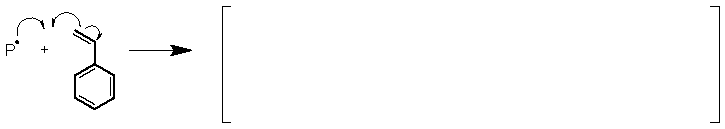
\includegraphics[width=\linewidth]{\figpath/Model2-styrene-tail.pdf}
				}\instructordisplay{
				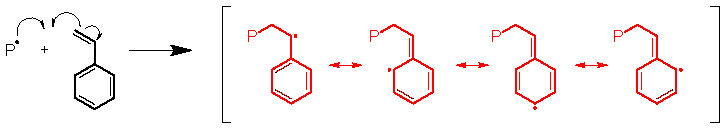
\includegraphics[width=\linewidth]{\figpath/Model2-styrene-tail-answer.pdf}
			}\end{solution}
			
				Draw the product expected from this reaction in the space above, making sure to include any relevant resonance structures.
				
				\vspace{12pt}
			\item Alternatively, the radical could have attacked the more-substituted side of the monomer (the ``head''), as shown below:
	
			\begin{solution}[1.2in]\studentdisplay{
				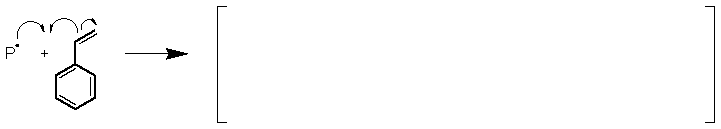
\includegraphics[width=\linewidth]{\figpath/Model2-styrene-head.pdf}
				}\instructordisplay{
				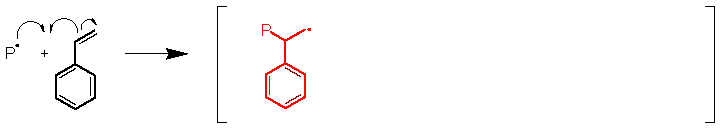
\includegraphics[width=\linewidth]{\figpath/Model2-styrene-head-answer.pdf}
			}\end{solution}
			
				Draw the product expected from this reaction in the space above, making sure to include any relevant resonance structures.
				
				\vspace{12pt}
			\item Based on your answers to the previous two parts, do you think it is more favorable for $P^\bullet$ to attack the head or the tail of the monomer?  Briefly defend your group's answer in 1-2 complete sentences.
				
				\begin{solution}[1.5in]
					It is more favorable for the radical to attack the tail of the monomer, because it produces a radical that is more resonance-stabilized.
				\end{solution}
		\end{enumerate}
		
		\question The different types of linkages that can be produced in a free-radical polymerization are summarized below (the linkage in question is shown with a dotted bond):
	
			\centerline{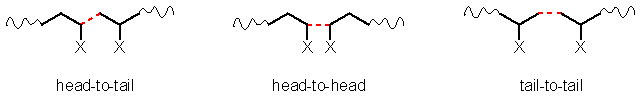
\includegraphics[scale=1.25]{\figpath/Model2-linkages.pdf}}
			
				Based on what you learned in the previous question, why does free-radical polymerization usually produce ``head-to-tail'' linkages?  Explain your team's reasoning in 2-3 complete sentences.
				
				\emph{Hint: you might find it useful to draw a few successive propagation steps, making sure that the monomers are correctly oriented based on what you learned in the previous question, and observe what type of linkage is formed and why.}
				
				\begin{solution}[2.75in]
					Because it is generally more favorable to attack the tail position, head-to-head linkages are unlikely.  Additionally, because attacking at the tail position puts the radical at the head position, we usually have a radical at the head of the chain attacking the tail of the next monomer, producing primarily head-to-tail linkages.
								
				\end{solution}
		
\end{ctqs}	

\begin{model}[Termination]
\label{\labelbase:mdl:FRPtermchem}

	The final step in a free-radical polymerization is \emph{termination}, in which polymer radicals are deactivated to form chains that cannot polymerize further.
	
	The two important termination mechanisms in free-radical polymerization are termination by \emph{combination}:
	
			\centerline{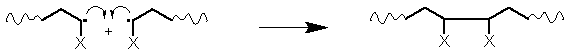
\includegraphics[scale=1.25]{\figpath/Model3-combination.pdf}}
	
	and termination by \emph{disproportionation}:
	
			\centerline{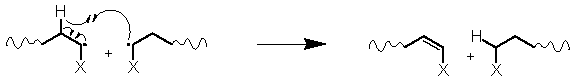
\includegraphics[scale=1.25]{\figpath/Model3-disprop.pdf}}

\end{model}

\begin{ctqs}

	\question How many polymer chains participate in each of the termination reactions shown in Model \ref{\labelbase:mdl:FRPtermchem}?
	
		\begin{solution}[0.5in]
			2 (they are bimolecular reactions)
		\end{solution}

	\question Why are the polymer chains on the right-hand side of each of these reactions considered to be ``dead'' chains that can no longer polymerize?
	
		\begin{solution}[1.25in]
			The polymer chains on the right-hand side of each of these reactions no longer have radicals on them, so they can no longer attack new monomers to add to the chain.
		\end{solution}
	
	\question Two propagating polystyrene radicals are shown below:
	
			\centerline{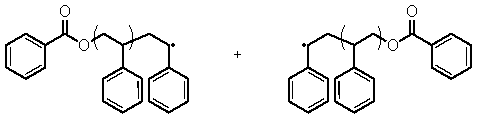
\includegraphics[scale=1]{\figpath/Model3-polystyrene.pdf}}
	
		\begin{enumerate}
			\item Draw the complete structure(s) of the product(s) formed if these radicals terminate by combination.
	
				\begin{solution}[1.25in]\instructordisplay{
					\centerline{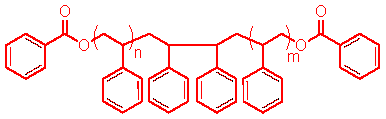
\includegraphics[scale=1]{\figpath/Model3-polystyrene-combination.pdf}}
				}\end{solution}
			
			\item What type of linkage is formed in the middle of the resulting polymer chain?
	
				\begin{solution}[0.25in]
					head-to-head
				\end{solution}
			
			\item How many initiator fragments does the resulting polymer chain contain?
	
				\begin{solution}[0.25in]
					2
				\end{solution}
			
			\item How is the length of the resulting polymer chain related to the length of the propagating radicals that participated in the termination reaction?
	
				\begin{solution}[0.5in]
					The polymer chain is twice as long as the radicals that participated in the termination reaction.
				\end{solution}
				
		\end{enumerate}
		
	\question For the same propagating polystyrene radicals discussed in the previous question,
	
		\begin{enumerate}
			\item Draw the complete structure(s) of the product(s) formed if these radicals terminate by disproportionation.
	
				\begin{solution}[1.5in]\instructordisplay{
					\centerline{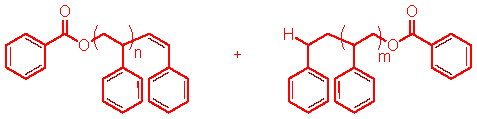
\includegraphics[scale=1]{\figpath/Model3-polystyrene-disproportionation.pdf}}
				}\end{solution}
			
			\item What type of functional group(s) are formed on the ends of the polymer chains?
	
				\begin{solution}[0.5in]
					a double bond on one and methylene (\ce{CH2}) on the other
				\end{solution}
			
			\item How many initiator fragments does each of the resulting polymer chains contain?
	
				\begin{solution}[0.5in]
					1
				\end{solution}
			
			\item How is the length of the resulting polymer chains related to the length of the propagating radicals that participated in the termination reaction?
	
				\begin{solution}[0.5in]
					The polymer chains are the same length as the propagating radicals that participated in the termination reaction.
				\end{solution}
				
		\end{enumerate}
	
	\question In 3-4 complete sentences, briefly summarize the key differences between polymers that terminate by combination and those that terminate by disproportionation.
	
				\begin{solution}[2.75in]
					Polymers that terminate by combination have a head-to-head linkage in the middle of the chain, which is absent from polymers that terminate by disproportionation.  Polymers that terminate by disproportionation have a new double bond on half of the terminated chain ends.  Polymers that terminate by combination also have two initiator fragments on each chain, while polymers that terminate by disproportionation only have one.  Finally, polymers that terminate by combination are twice as long as the propagating radicals, while polymers that terminate by disproportionation are the same length as the propagating radicals.
				\end{solution}
	

\end{ctqs}

		

\begin{model}[Chain Transfer]
\label{\labelbase:mdl:FRPxferchem}

	A side reaction that can often occur during free radical polymerization is a ``transfer'' of the radical from the propagating chain to another molecular species, such as solvent.  This process is called \emph{chain transfer}.
	
	An example chain transfer reaction is shown below:
	
			\centerline{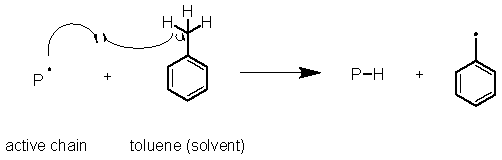
\includegraphics[scale=1.25]{\figpath/Model4-xfertoluene.pdf}}
	
\end{model}

\begin{ctqs}
	\question Explain, in 1-2 complete sentences, why we might say that chain transfer \emph{effectively} terminates the growing polymer chain:
	
		\begin{solution}[1.75in]
			The chain transfer reaction takes an active chain and essentially caps the radical with a hydrogen atom.  Because the chain no longer has a radical on it after this reaction takes place, it can no longer attack new monomers, so has effectively been terminated.
		\end{solution}
	
	\question Qualitatively, do you expect chain transfer to result in an increase, decrease, or no change in the molecular weight of the polymers produced in a free radical polymerization?  Briefly explain your reasoning.
	
		\begin{solution}[1.75in]
			Chain transfer should decrease the molecular weight of the polymers produced in a free radical polymerization, for two reasons.  First, it effectively terminates chains before they would otherwise stop growing, so the chains end up being shorter.  Second, IF the new radical can act as an initiator to start new chains, the monomers will end up being distributed over a larger number of chains, reducing the average molecular weight.
		\end{solution}
		
\end{ctqs}


\begin{exercises}

	\exercise Indicate whether you expect each of the following factors to promote or inhibit formation of products in the reactions shown in Model \ref{\labelbase:mdl:FRPinitchem}, and briefly identify why: %Note: removed this one from Model 1, but I still like it
	
		\begin{enumerate}
			\item Energy required to break chemical bonds
	
				\begin{solution}
					It is energetically costly to break chemical bonds, so the high energy cost of doing so inhibits formation of the radical products.
				\end{solution}
			
			\item Increase in the number of molecules present
	
				\begin{solution}
					Increasing the number of molecules is generally entropically favorable, so should promote formation of the radical products.
				\end{solution}
			
			\item Formation of a gaseous byproduct
	
				\begin{solution}
					Gaseous byproducts can escape the solution (and potentially be removed under vacuum or bubbling inert gas).  Removing the gaseous byproduct pulls the reaction to the right, per Le Chatelier's principle, and promotes formation of the radical products.
				\end{solution}
			
			\item Formation of resonance-stabilized products
	
				\begin{solution}
					Forming resonance-stabilized products makes formation of products energetically more favorable, so promotes formation of the radical products.
				\end{solution}
		\end{enumerate}
		
		Using your responses to the above questions, explain in 2-3 complete sentences why both of the initiators shown in \ref{\labelbase:mdl:FRPinitchem} decompose to form radicals when they are heated.
		
	
				\begin{solution}
					Heating the reaction mixture provides the energy necessary to drive homolytic cleavage of the necessary bond(s).  Once this energy is provided, formation of the radicals follows because the products are entropically and enthalpically favorable.
				\end{solution}

	\exercise Draw the structure of a chain of poly(methyl methacrylate) prepared by free radical polymerization using AIBN as the initiator, assuming that all termination is by combination.  Make sure to show all relevant features of the polymer structure.
	
		\begin{solution}\instructordisplay{
				\centerline{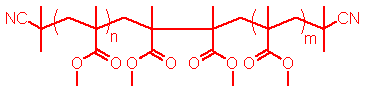
\includegraphics[scale=1.25]{\figpath/exercises-PMMAcomb-answer.pdf}}
		}\end{solution}
	
	\exercise In Model \ref{\labelbase:mdl:FRPxferchem}, you considered chain transfer to solvent (toluene).  However, chain transfer can also take place between a radical chain and other molecular species in the reaction, which can have important consequences.
	
		\begin{enumerate}
			%\item Complete the following reaction scheme for chain-transfer to monomer:
			
			\item Complete the following reaction scheme for chain-transfer to polymer:
	
			\begin{solution}\studentdisplay{			
				\centerline{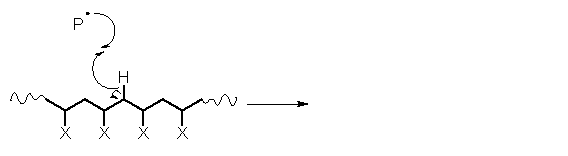
\includegraphics[scale=1.25]{\figpath/exercises-xferpolymer.pdf}}
				}\instructordisplay{		
				\centerline{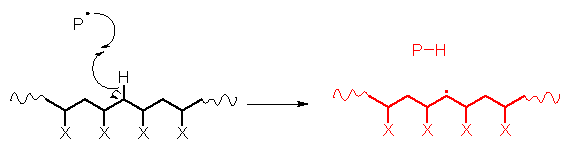
\includegraphics[scale=1.25]{\figpath/exercises-xferpolymer-answer.pdf}}
			}\end{solution}
			
			\item If the resulting radical species in part (b) then started adding additional monomers, what type of polymer architecture(s) could result?
			
				\begin{solution}\instructordisplay{
					Sketching out the resulting structure, we see that we obtain a branched polymer.
					
									\centerline{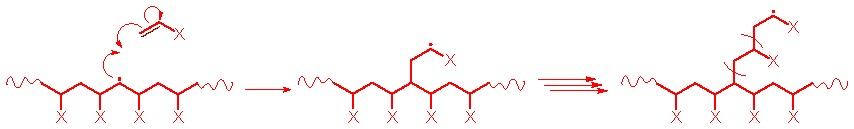
\includegraphics[width=\textwidth]{\figpath/exercises-xferpolymer-answer2.pdf}}
				}\end{solution}
		\end{enumerate}
		
		% potential additional topic for exercises:
		% 1) which monomers can and cannot be polymerized (DOI 10.1007/978-3-642-38730-2_7 has useful information about polypropylene, for example, though it may belong better in the kinetics activity
		% 2) role of oxygen in FRP (e.g its inhibition mechanism)
	
\end{exercises}


%\begin{problems}
%
%	\problem First exercise
%	\problem Second exercise
%	
%\end{problems}


	
\end{activity}


\end{document}
